%packages
\documentclass{article}
\usepackage{graphicx}
\usepackage{titlesec}
\usepackage{fancyhdr}
\usepackage[margin=0.6in]{geometry}
\usepackage[UKenglish]{babel}% http://ctan.org/pkg/babel
\usepackage[UKenglish]{isodate}% http://ctan.org/pkg/isodate
\usepackage[T1]{fontenc}
\usepackage{blindtext}
\usepackage{sectsty}
\usepackage{float}
\usepackage{caption}



\pagestyle{fancy}
\fancyhf{}
\rhead{For HEAnet CLG}
\chead{Cooperative Education Report}
\lhead{\today}
\rfoot{Page \thepage}
\lfoot{By Barth O'Keeffe}
\cfoot{Student number : 14180847   }
\titleformat{\section}{\Large\bfseries}
\titleformat{\section}{\center\bfseries}
\sectionfont{\fontsize{12}{15}\selectfont}

%custom commands
\newcommand\tab[1][4.7cm]{\hspace*{#1}}


\begin{document}
\begin{titlepage}
	\begin{center}
		\begin{figure}
			
\includegraphics[width=500pt,height=100pt,]{ul_logo.png}
		\end{figure}
	\end{center}
	\begin{center}
		\begin{LARGE}
			COOPERATIVE EDUCATION REPORT \\
		\end{LARGE}
	\end{center}
	\begin{Large}
		
		Date: \today  \\
		
		Student Name: Barth O'Keeffe\\
		
		ID Number: 14180847\\
		
		Course: Mobile Communications and Security \\
		
		Employer Name: HEAnet CLG\\
		
		Employer Address: HEAnet CLG,\\
		\tab 1st Floor,\\
		\tab 5 George's Dock,\\
		\tab IFSC,\\
		\tab Dublin 1\\
		
		
		Start Date of placement:\\
		
		End Date of placement:\\
		
		Name of Company Supervisor('s):\\
		
		Company Supervisor's Position:\\
		
		Signature of Company Supervisor('s):\\
		
		Company Stamp:\\
		
		Name of Visiting University Staff Member:\\
	\end{Large}
\end{titlepage}
\tableofcontents
\newpage
\section{Summary of Placement (min. 1 page)}
\subsection{Induction}
Upon arrival at HEAnet I met with my line manager Brian McArdle, with whom I completed my induction with. As part of my induction I had to attend various meetings with Brian and other members of HEAnet staff (HR and HEAnets Health and safety officer). The purpose of the induction meetings is to inform new staff of the work that is carried out by HEAnet's various teams, whats expected of the as a HEAnet employee in terms of personal conduct,working hours and what to do in the event of an emergency (such as a fire). I also had to complete a manual handling course and was briefed on HEAnets acceptable usage policy as regards the internet for personal use.

Once my general induction had been my next task was to set up my desktop on the advice of Brian I installed replaced Windows 10 with Ubuntu 16.04 (a Linux distribution), which I had previous experience with from several modules I had taken as part or my degree. The next step was to set up the various accounts I needed
\newpage
\section{Brief history of the HEAnet CLG (min. 1 page)}

\paragraph{What is HEAnet?}
HEAnet is Ireland's national education and research network. It has been in operation since 1983 as a collaborative endeavour between its member institutions. From 1993 until the end of 1997, the network services were managed by UCD Computing Services, under contract to HEAnet. In November 1997, HEAnet was incorporated as a company limited by guarantee, and relocated its network operations centre to Marine House, Mount St, Dublin 2. In 2001, HEAnet moved to Brooklawn House, Shelbourne Road, Dublin 4. In July 2006, the company moved to new offices at 5, George's Dock, I.F.S.C, Dublin 1, D01 X8N7.

\paragraph{HEAnet Today}

HEAnet's very high bandwidth network connects all Irish Universities, all Institutes of Technology, other higher education institutions (HEIs) and research organisations, in addition to all primary and post-primary schools across Ireland.

HEAnet's e-Infrastructure services underpin academic research and education activity in Ireland with approximately 200,000 students and staff (third-level) and approximately 800,000 students and staff (first and second-level) relying on the HEAnet network each day for their learning and research needs.

These institutions are linked in a state-of-the art wide area network (WAN) spanning the country. Significantly, HEAnet played a key role in the establishment of the Irish Neutral Exchange (INEX), a facility which enables all Irish Internet service providers (ISPs) to exchange their Internet traffic in Ireland. As a result, HEAnet members benefit from a high level of connectivity with all other major Irish networks, while customers of the commercial ISPs enjoy a high level of connectivity with the national education and research network. HEAnet currently connects to INEX with 2 x 10 Gbit/s links.

HEAnet also provides connections to networks in Europe by means of its 2 x 10 Gbit/s link with the GÉANT backbone, and 2 x 10 Gbit/s circuit links HEAnet to Janet, the UK education and research network. HEAnet has a 2 x 10 Gbit/s connection to the General Internet. HEAnet also funds and manages the National Information Server (ftp.heanet.ie) which serves as an online repository of information resources of relevance to the academic and research community, both in Ireland and around the globe. HEAnet also hosts a number of major dataset services for the education and research community. Through the provision of state-of-the-art network and communications technology, and important Web-based information services, HEAnet has and will continue to promote progress in today's Information Society.

\paragraph{Mission Statement}
"To realise Ireland's education and research goals in partnership with our clients by providing advanced infrastructure and services."
\paragraph{HEAnet's vision is:}
\begin{itemize}
	\item Be a collaborative partner who is intrinsic to the business needs of our clients:
	      \begin{itemize}
	      	\item Continue to be the trusted provider of networking and infrastructure services.
	      	\item Be the preferred broker of cloud and other services to our clients.
	      	\item Be the link that facilitates clients to collaborate on innovative solutions.
	      \end{itemize}
	\item Be recognised for fast, agile and efficient delivery of shared services.
	\item Be the driver of Identity Federation across the education and research sector and into the wider public service.
	\item Continue to be a key provider of cost-effective procurement for the education and research sector.
	\item Be a key advisor in the development and emergence of new and disruptive technologies.
	\item Be the conduit to Europe for the promotion of Irish education and research interests and the trusted gateway to world-wide infrastructural services.
	\item Be recognised as an excellent place to work.
\end{itemize}
\begin{figure}[H]
	\centering
	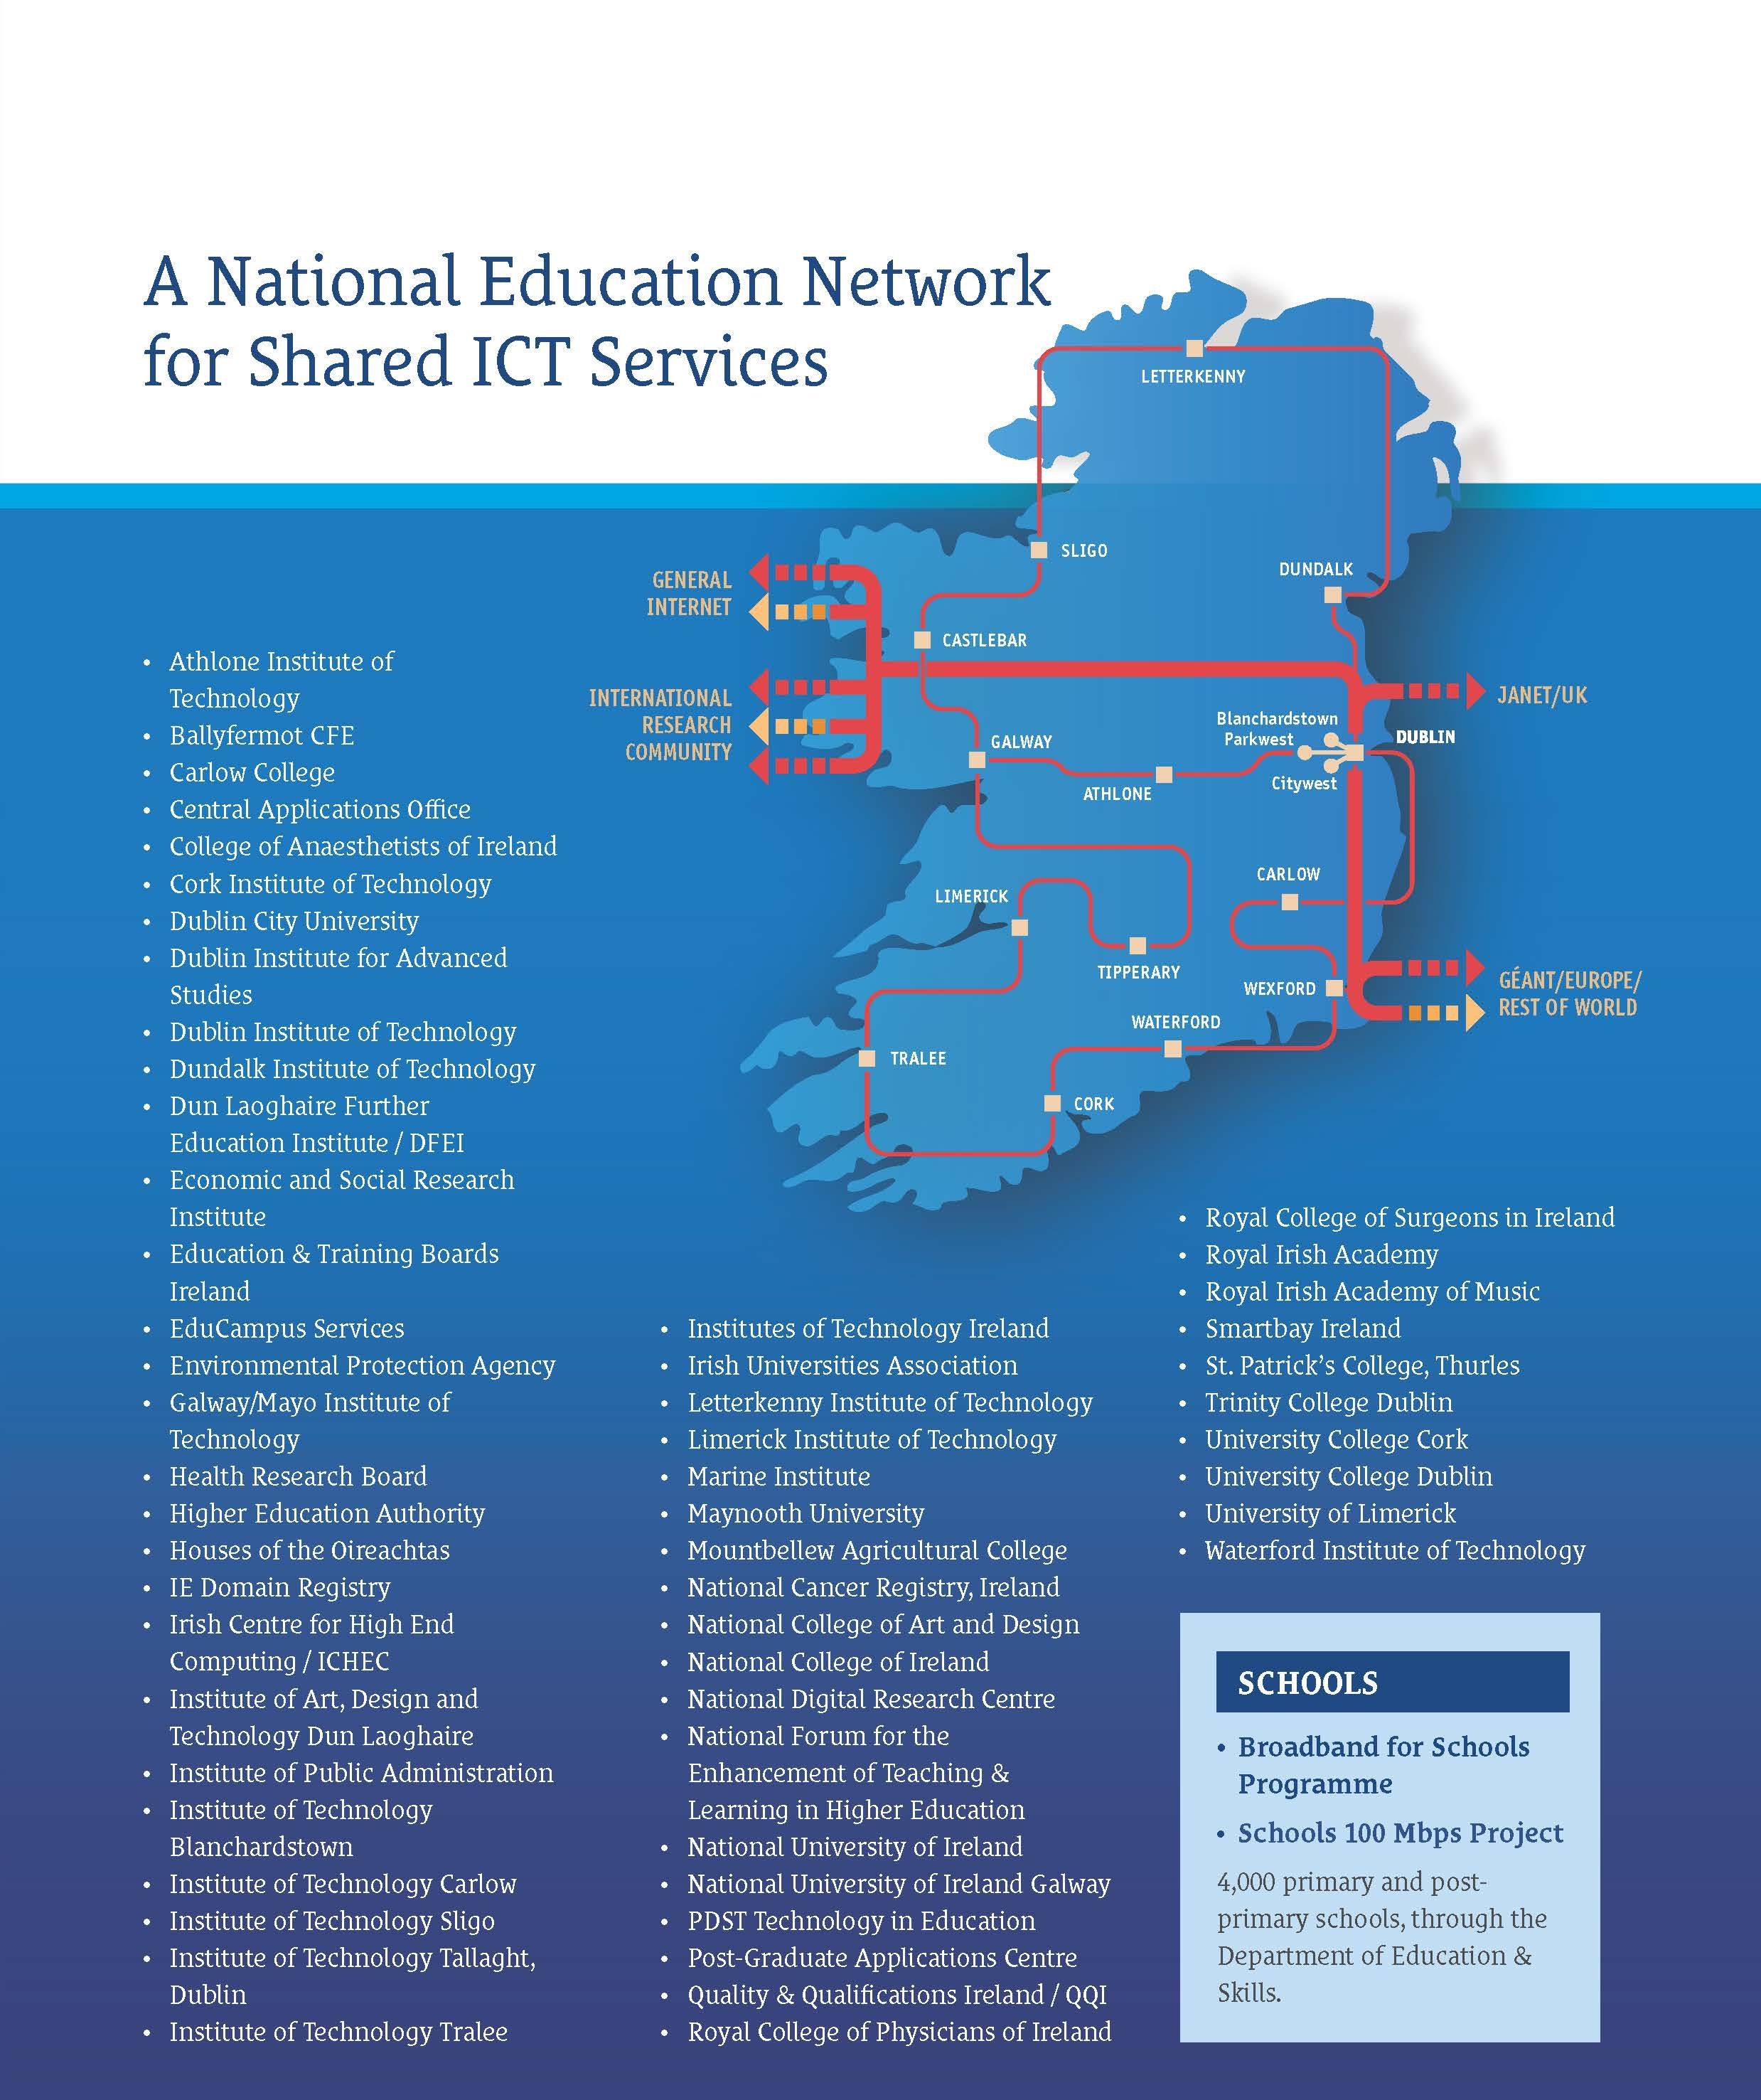
\includegraphics[width=450pt,height=450pt,]{HEAnet-Infrastructure-Client-Map-Nov-2015.jpg}
	\captionof{figure}{Map of HEAnets network}\label{HEAnet-Infrastructure-Client-Map-Nov-2015.jpg}
\end{figure}

\newpage

\section{Structure of the organisation (Teams)(min. 1 page)}
\subsection{Overview}
\begin{figure}[H]
	\centering
	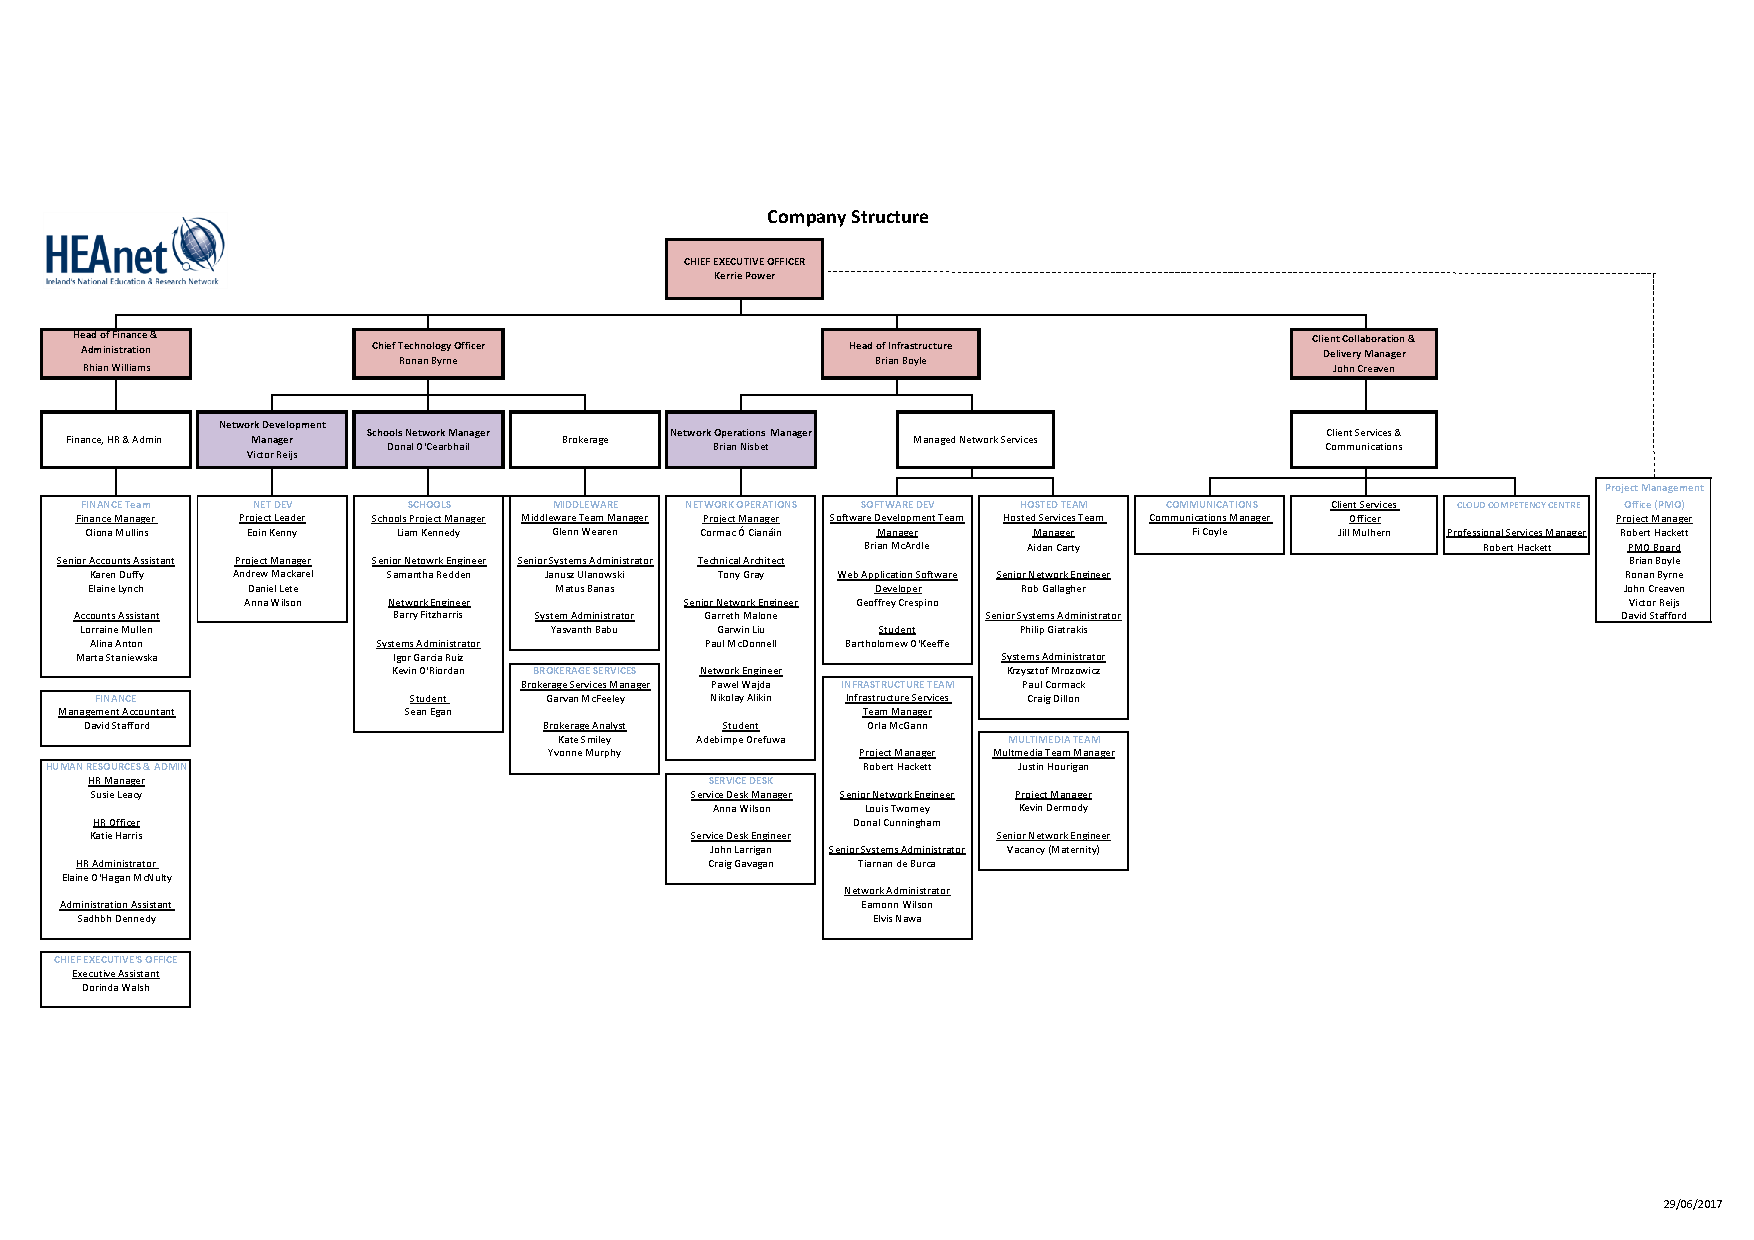
\includegraphics[width=550pt,height=550pt,]{Company Structure - Jul-17.pdf}
	\captionof{figure}{Company Structure}\label{Company Structure - Jul-17.pdf}
\end{figure}
\subsection{Client Communications}
\subsection{Brokerage}
\subsection{Net Dev}
\subsection{Service Desk}
\subsection{Software Development Team}
\paragraph{Areas of responsibility \newline}
The SWDEV team consists of two full time developers.
More people may be involved on a per project basis, with the developers forming the core and determining policies, tool sets and work practices for software within HEAnet.
The role of the SWDEV group is to ensure that HEAnet has the capabilities to configure, maintain and where appropriate, build the required tools for delivery of services to our clients. While the initial requirements are for tools for the NOC, it is hoped that this will broaden in scope after a time.
\subsection{Net Ops}
\subsection{Middleware}
\paragraph{Areas of responsibility \newline}
Middleware is primarily responsible for Identity and Access Management (IAM). For example when a Ul student log's in to an online resource such as ACM Digital Library via shibboleth (Edugate (Federated Access)) using their Ul credentials, this service is provided by Middleware.
\begin{itemize}
	\item \textbf{24 x 7  on-call support}
	      \begin{itemize}
	      	\item HEAnet's Managed, Hosted and Standby Shibboleth IdP Service has been extended to include out of hours support. This enables HEAnet to meet its 99.95\% service uptime target by extending proactive and reactive support outside HEAnet's normal business hours of 9:00am to 5:30pm Monday to Friday. In the event of a Priority 1 or 2 Incident, HEAnet will act to resolve such issues and will be provide clients with a detailed Reason For Outage report within 5 working days of the incident.
	      \end{itemize}
	\item \textbf{Edugate (Federated Access)}
	      \begin{itemize}
	      	\item Edugate is HEAnet's federated access service. Edugate's purpose is to eliminate the need for multiple user-names and passwords, which inconveniences users. Federated access means just a single set of credentials is required to log into a range of services.
	      \end{itemize}
	\item \textbf{Hosted and Standby SAML Identity Provider}
	      \begin{itemize}
	      	\item This service will process SAML authentication requests on HEAnet infrastructure when HEAnet detects that the primary SAML Identity Provider service is unavailable on campus. The service includes Active Directory replication via VPN tunnel, the Identity Provider is based on Shibboleth or Microsoft Active Directory Federation Services.
	      \end{itemize}
	\item \textbf{JAGGER (Resource Registry 3)}
	      \begin{itemize}
	      	\item 	Jagger (ResourceRegistry3) is developed by HEAnet to manage the Edugate multiparty SAML federation. Other organisations use Jagger to manage their federations but it can be used to manage the web-of-trust for a single entity. It can also be used a a GUI for the Shibboleth SAML Identity Provider (www.shibboleth.net)
	      \end{itemize}
	\item \textbf{Managed SAML Identity Provider}
	      \begin{itemize}
	      	\item HEAnet's Managed SAML Identity Provider service provides remote monitoring and management of an institutions Shibboleth Identity Provider, this management extends to multiple instances whether on-campus or hosted by HEAnet. The service is designed to allow an institution to rely on HEAnet's expertise for troubleshooting Shibboleth Identity Provider issues or planning for campus directory changes or co-ordination with new SAML service providers who are not Edugate compliant.
	      \end{itemize}
	      \newpage
	\item \textbf{SAML Identity Provider Services}
	      \begin{itemize}
	      	\item \textbf{Shibboleth Identity Provider Upgrade}\\
	      	      Institutions who wish to upgrade their Identity Provider service between one major version and a subsequent version can follow guides provided by the Shibboleth consortium or avail of this HEAnet service. HEAnet will upgrade existing deployments ensuring customisations such as login pages, attribute resolution scripts or attribute release customisations are ported to the latest Shibboleth version. Prices vary by the number of Shibboleth nodes deployed and the number of bilateral services configured (if any).coop.pub
	      	\item \textbf{Bilateral SAML Configurations}\\
	      	      HEAnet will engage with services providers to join Edugate and assist institutions availing of such member services at no charge to the institution. Where service providers do not wish to join Edugate and support SAML, HEAnet can configure a bilateral trust between the institutions identity provider service and the service provider. HEAnet has configured bilateral configurations for the services below:
	      	      \begin{itemize}
	      	      	\item Google Apps for Education
	      	      	\item Office 365 (incl. Yammer and Azure)
	      	      	\item Adobe Creative Cloud
	      	      	\item Amazon Web Services
	      	      	\item Ezproxy
	      	      	\item Sharepoint
	      	      	\item TCS iON
	      	      	\item Teamwork.com
	      	      	\item Freshdesk.com
	      	      	\item Workday.com
	      	      	\item Athens
	      	      	      
	      	      \end{itemize}
	      	\item \textbf{Active Directory Federation Services integration with Edugate}\\
	      	      Microsoft's ADFS can provide a compatible identity provider services for Edugate. HEAnet can integrate an on-premise ADFS server with Edugate to ensure users can logon to Edugate member services via ADFS.
	      \end{itemize}
\end{itemize}
\subsection{Multimedia}
\subsection{Hosted Services}
\subsection{Schools}
\subsection{Finance, Admin and HR}
\subsection{Infrastructure Services Team}
\paragraph{Areas of responsibility}
\begin{itemize}
	\item Data centres (Blanchardstown PoP, Parkwest PoP, Waterford Data centre(TSSG))
	\item Data centre hosting (formerly known as colocation)
	\item Services Network
	\item eduroam
	\item Edustorage
	\item Ciera (IaaS Cloud)
	\item LAN Support
	\item Educampus-Support-Services
\end{itemize}


\newpage

\section{Student's main responsibilities(min. 2 page)}

\newpage

\section{Opportunities for Learning during Co-op(min. 4 page)}
\subsection{Basic Work Skills}

\subsection{Communication Skills}
\subsection{Problem Solving Skills}
\subsection{Interpersonal and Teamwork Skills}
\subsection{Cultural/International Awareness}
Under Cultural/International awareness, you could talk about the different nationalities who work in HEAnet (Polish, Russian, Indian, Greek, South African, Spanish, Dutch,Slovak) about 20 percent of the org were not born in Ireland as far as I can tell. You could put a section on HEAnet's international relations (e.g. Geant membership;  6 HEAnet staff are working on Geant activities with their counterparts in other NRENs).
\subsection{ICT Skills}
\subsection{Organisational Awareness}
\subsection{Professional Skills}
In the course of my placement I had the opportunity to learn several new technology's including Git, Docker, Linux system administration, Continuous Integration, Markdown, Node Package Manager (npm) and JavaScript (CasperJS).
I also had the opportunity to improve some of my existing skills such as PHP, MySQL, Linux shell scripting (bash) and front end web development.
\subsubsection{Git}
\paragraph{What is Git?}
Git is a version control system (VCS) for tracking changes in computer files and coordinating work on those files among multiple people. It is primarily used for source code management in software development, but it can be used to keep track of changes in any set of files. As a distributed revision control system it is aimed at speed, data integrity and support for distributed, non-linear work flows.
\paragraph{How is it used at HEAnet}
\subsubsection{Docker}
\paragraph{What is Docker?}
Docker is a software technology providing containers, promoted by the company Docker Inc. Docker provides an additional layer of abstraction and automation of operating-system-level virtualization on Windows and Linux. Docker uses the resource isolation features of the Linux kernel such as cgroups and kernel namespaces, and a union-capable file system such as OverlayFS and others to allow independent "containers" to run within a single Linux instance, avoiding the overhead of starting and maintaining virtual machines.
\subsubsection{Linux system administration}
\subsubsection{Continuous Integration}
\paragraph{What is Continuous Integration?}
Continuous Integration (CI) is a development practice that requires developers to integrate code into a shared repository several times a day. Each check-in is then verified by an automated build. By integrating regularly, you can detect errors quickly, and locate them more easily.
\subsubsection{Markdown}
\paragraph{What is Markdown?}
Markdown is a lightweight markup language with plain text formatting syntax. It is designed so that it can be converted to HTML and many other formats using a tool by the same name.[8] Markdown is often used to format readme files, for writing messages in online discussion forums, and to create rich text using a plain text editor. As the initial description of Markdown contained ambiguities and unanswered questions, many implementations and extensions of Markdown appeared over the years to answer these issues.
\subsubsection{Node Package Manager (npm)}
\paragraph{What is npm?}
Node Package Manager (npm) is a package manager for the JavaScript programming language. It is the default package manager for the JavaScript runtime environment Node.js. It consists of a command line client, also called npm, and an online database of public packages, called the npm registry. The registry is accessed via the client, and the available packages can be browsed and searched via the npm website.
\subsubsection{JavaScript (CasperJS)}
\paragraph{What is JavaScript?}
JavaScript often abbreviated as JS, is a high-level, dynamic, weakly typed, object-based, multi-paradigm, and interpreted programming language. Alongside HTML and CSS, JavaScript is one of the three core technologies of World Wide Web content production. It is used to make web-pages interactive and provide online programs, including video games. The majority of websites employ it, and all modern web browsers support it without the need for plug-ins by means of a built-in JavaScript engine. Each of the many JavaScript engines represent a different implementation of JavaScript, all based on the ECMAScript specification, with some engines not supporting the specification fully, and with many engines supporting additional features beyond ECMA.

As a multi-paradigm language, JavaScript supports event-driven, functional, and imperative (including object-oriented and prototype-based) programming styles. It has an API (Application Programming Interface) for working with text, arrays, dates, regular expressions, and basic manipulation of the DOM, but does not include any I/O, such as networking, storage, or graphics facilities, relying for these upon the host environment in which it is embedded.

Initially only implemented client-side in web browsers, JavaScript engines are now embedded in many other types of host software, including server-side in web servers and databases, and in non-web programs such as word processors and PDF software, and in runtime environments that make JavaScript available for writing mobile and desktop applications, including desktop widgets.

Although there are strong outward similarities between JavaScript and Java, including language name, syntax, and respective standard libraries, the two languages are distinct and differ greatly in design; JavaScript was influenced by programming languages such as Self and Scheme.

\paragraph{What is CasperJS?}
CasperJS is a navigation scripting and testing utility for PhantomJS and SlimerJS (still experimental). It eases the process of defining a full navigation scenario and provides useful high-level functions and methods for doing common tasks such as:
\begin{itemize}
	\item defining and ordering navigation steps
	\item filling forms
	\item clicking links
	\item capturing screen-shots of a page (or an area)
	\item making assertions on remote DOM
	\item logging and events
	\item downloading resources, even binary ones
	\item catching errors and react accordingly
	\item writing functional test suites, exporting results as JUnit XML (xUnit)
\end{itemize}
\begin{center}
	
\end{center}

\subsubsection{PHP}
\subsubsection{MySQL}
\subsubsection{Linux shell scripting (bash)}
\subsubsection{Front end web development}


\end{document}
